\documentclass{article}
\usepackage{polski}
\usepackage[utf8]{inputenc}
\usepackage[OT4]{fontenc}
\usepackage{graphicx,color}
\usepackage{url}
\usepackage[pdftex,hyperfootnotes=false,pdfborder={0 0 0}]{hyperref}
\usepackage{float}

\begin{document}
\thispagestyle{empty} %bez numeru strony

\begin{center}
{\large{Sprawozdanie z laboratorium:\\
Informatyka w Medycynie}}

\vspace{3ex}

Tomograf

\vspace{3ex}
{\footnotesize\today}

\end{center}


\vspace{10ex}

Prowadzący: Iwo Błądek

\vspace{5ex}

Autorzy:
\begin{tabular}{lllr}
\textbf{Adam Pioterek} & inf122446 & adam.pioterek@student.put.poznan.pl \\
\textbf{Marcin Drzewiecki} & inf122472 & marcin.drzewiecki@student.put.poznan.pl \\
\end{tabular}

\newpage



\section{Algorytm}
\begin{description}
\item[1)] Wczytujemy obraz, konwertujemy do skali szarości.
\item[2)] Wybieramy liczbę emiterów, krok, liczbę receptorów przypadającą na jeden emiter, rozwartość kątową.
\item[3)] Dla każdej projekcji emiter-receptor za pomocą algorytmu Bresenhama wyznaczamy piksele należące do linii. Dla każdej linii wyznaczamy średnią wartość pikseli leżących na niej. W ten sposób uzyskujemy sinogram.
\item[4)] Na podstawie sinogramu odtwarzamy obraz: dla każdego elementu sinogramu (projekcji emiter-receptor) dodajemy do wartości piksela średnią wartość piksela odczytaną z tablicy. 
\item[5)] Wpisujemy wyniki do tablicy wynikowej reprezentującej obraz, normalizujemy wartości pikseli oraz stosujemy filtr uwzględniający gęstość linii przechodzących przez dany obszar obrazu[1]
\item[6)] Zapisujemy obraz oraz proces jego odtwarzania.
\end{description}
 
\section{Wynik działania programu}
Poniżej znajdują się sinogramy dla obrazów wejściowych uzyskane za pomocą transformacji Radona oraz obrazy odtworzone z sinogramu za pomocą odwrotnej transformacji Radona. Obrazy są przedstawione w kolejności: sinogram, uzyskany obraz bez filtracji i z filtracją. Po lewej zawsze widoczny jest obraz wejściowy.

\begin{figure}
\begin{center}
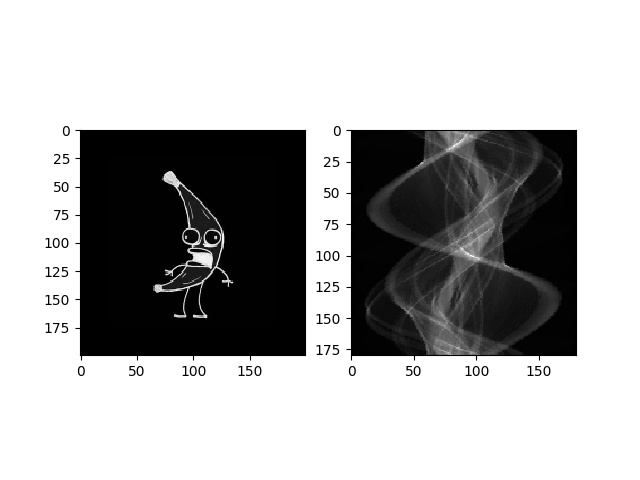
\includegraphics[width=0.8\textwidth]{./banana/sinogram.jpg}
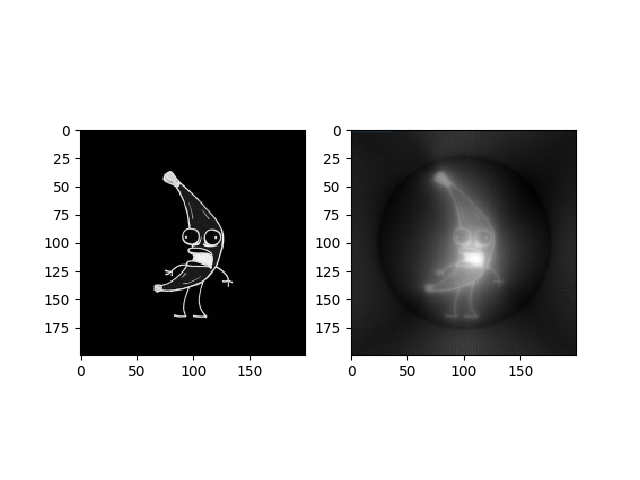
\includegraphics[width=0.8\textwidth]{./banana/reconstructedImg.png}
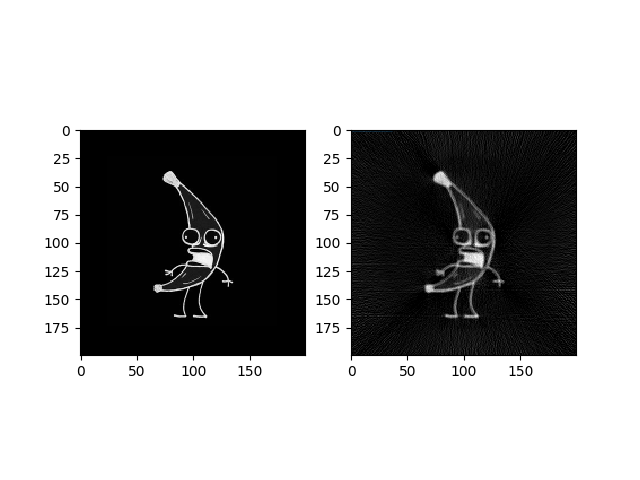
\includegraphics[width=0.8\textwidth]{./banana/reconstructedImg2.png}
\end{center}
\end{figure}

\begin{figure}
\begin{center}
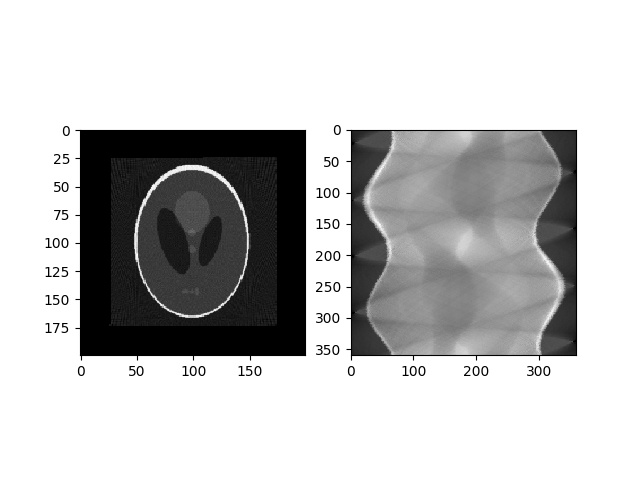
\includegraphics[width=0.8\textwidth]{./phantom/sinogram.jpg}
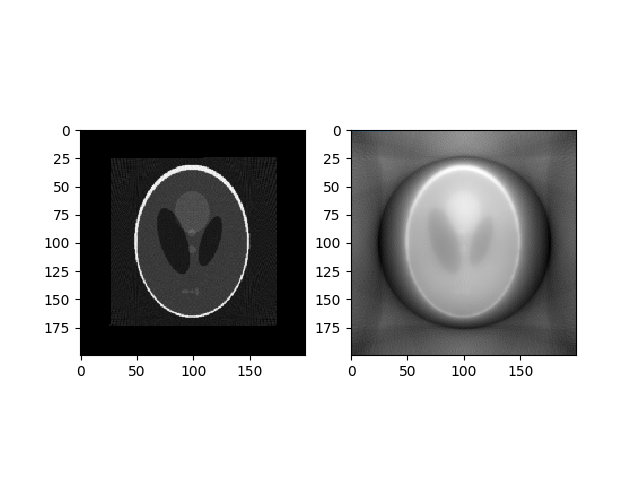
\includegraphics[width=0.8\textwidth]{./phantom/reconstructedImg.png}
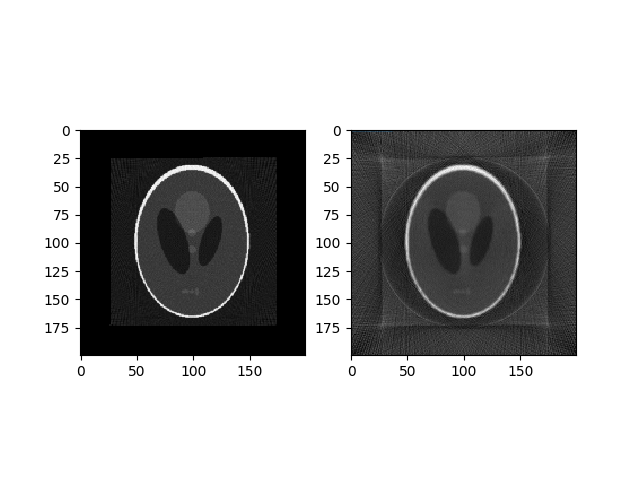
\includegraphics[width=0.8\textwidth]{./phantom/reconstructedImg2.png}
\end{center}
\end{figure}

\begin{figure}
\begin{center}
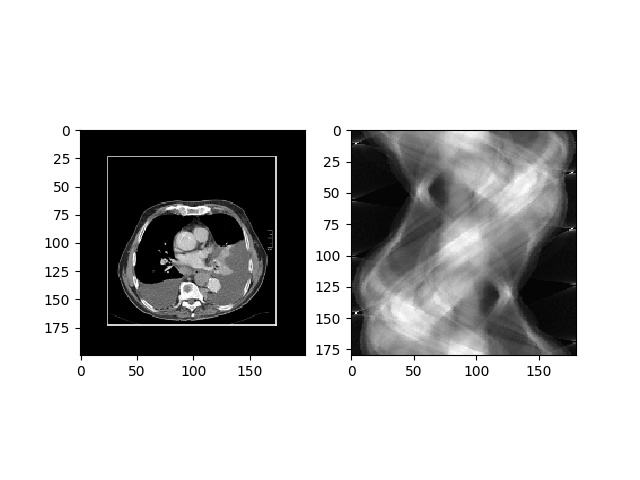
\includegraphics[width=0.8\textwidth]{./something/sinogram.jpg}
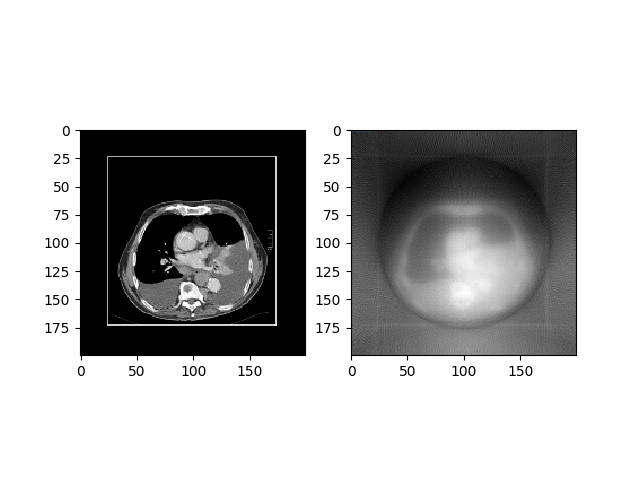
\includegraphics[width=0.8\textwidth]{./something/reconstructedImg.png}
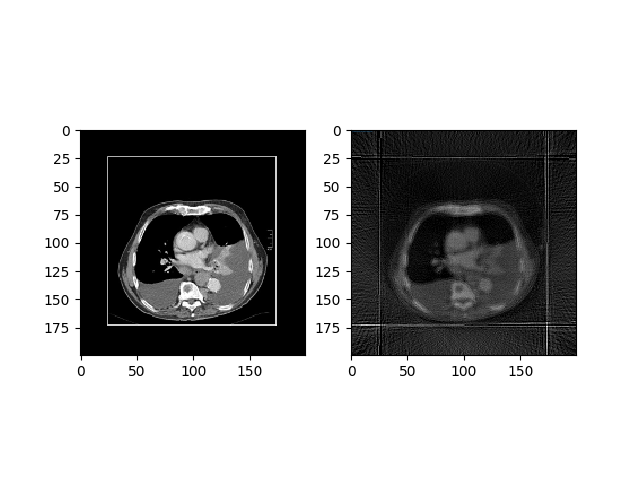
\includegraphics[width=0.8\textwidth]{./something/reconstructedImg2.png}
\end{center}
\end{figure}

\begin{figure}
\begin{center}
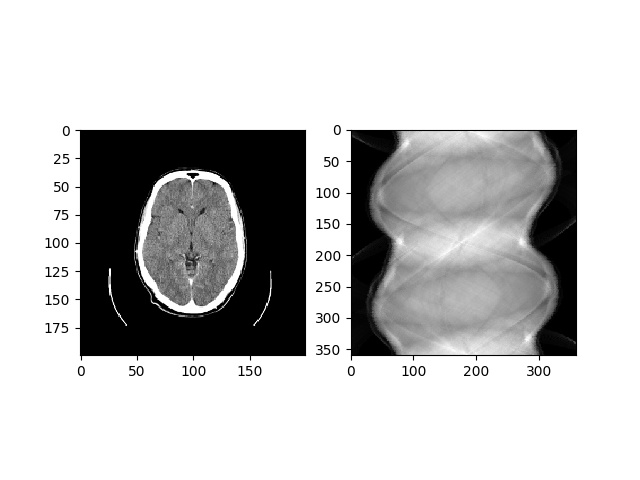
\includegraphics[width=0.8\textwidth]{./brain/sinogram.jpg}
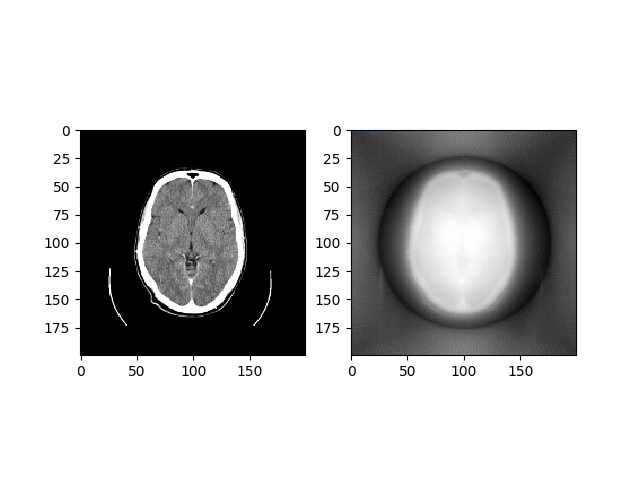
\includegraphics[width=0.8\textwidth]{./brain/reconstructedImg.png}
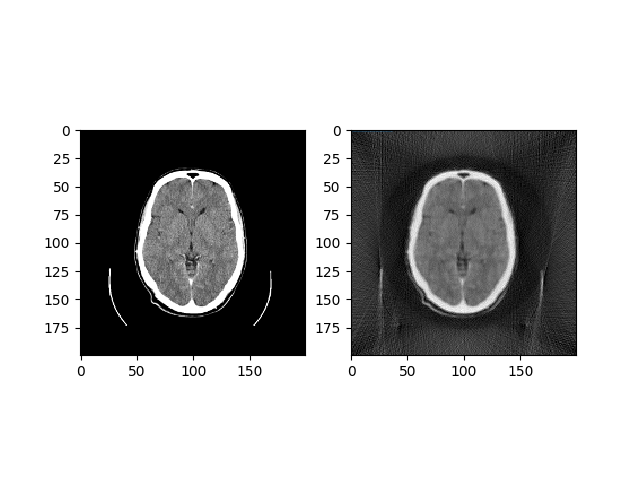
\includegraphics[width=0.8\textwidth]{./brain/reconstructedImg2.png}
\end{center}
\end{figure}

\newpage
\section{Analiza parametrów}

Zbadaliśmy zależność błędu (średniokwadratowego) mierzonego na podstawie różnicy wartości pikseli obrazu wejściowego (phantom) oraz uzyskanego na wyjściu od: rozpiętości kątowej, kroku układu emiter-detektor, liczby detektorów przypadających na jeden emiter. Badaliśmy błąd zarówno dla zastosowanego filtru, jak i bez niego.

\subsection{Rozpiętość kątowa}
\begin{figure}[H]
\begin{center}
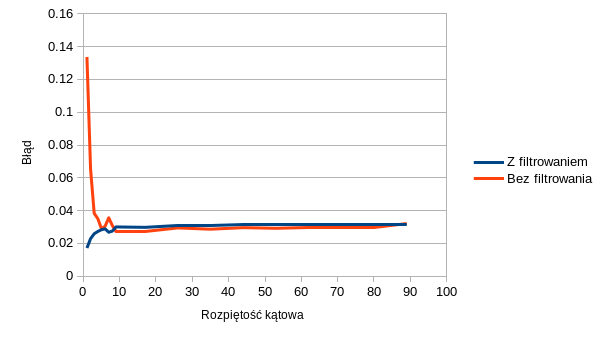
\includegraphics[width=0.8\textwidth]{./width.png}
\end{center}
\end{figure}

Wykres przedstawia zależność błędu od rozpiętości kątowej mierzonej w stopniach przy stałych pozostałych parametrach. Im większa jest rozpiętość, tym mniejszy błąd. Dla wersji bez filtrowania największą różnicę można zauważyć dla wartości z przedziału 0-10 stopni. Nic nie można powiedzieć dla wersji z filtrowaniem. Najprawdopodobniej zaobserwowane wartości są przekłamane. Przy stosunkowo dużej rozpiętość kątowej nie ma znaczącej różnicy w wersji z filtrowaniem i bez. 

\subsection{Krok układu emiter-detektor}
\begin{figure}[H]
\begin{center}
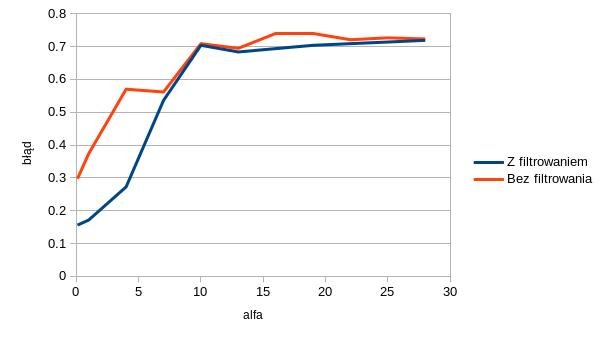
\includegraphics[width=0.8\textwidth]{./alpha.jpg}
\end{center}
\end{figure}

Wykres przedstawia zależność błędu od kroku układu emiter-detektor. Oprócz wzrostu błędu wraz ze wzrostem kroku, istotny jest fakt, że przy zmniejszającym się kroku w wersji bez filtrowania nie da się osiągnąć tak dobrej dokładności odwzorowania jak w wersji z filtrowaniem. Zmniejszanie kroku poniżej wartości $0,1$ niosło za sobą duży wzrost wymaganej liczby obliczeń, dlatego nie zostały one wykonane. Można przypuszczać, że dla mniejszych wartości wartość nie osiągnie $0$ ze względu na błędy w obliczeniach zmiennoprzecinkowych. 

\subsection{Liczba detektorów przypadająca na jeden emiter}
\begin{figure}[H]
\begin{center}
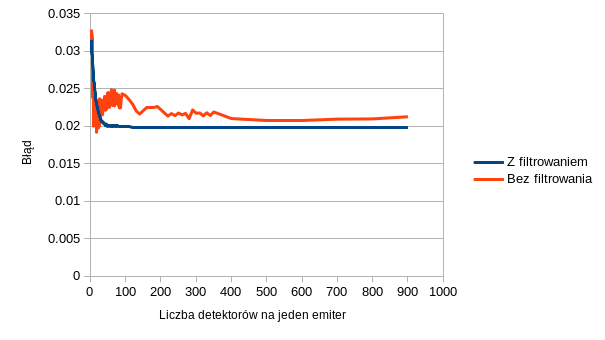
\includegraphics[width=0.8\textwidth]{./detector_count.png}
\end{center}
\end{figure}

Wykres przedstawia zależność błędu od liczby detektorów przypadających na jeden emiter. Podobnie, jak w przypadku poprzedniej analizy, największy spadek błędu występuje dla małej liczby detektorów na jeden emiter. Wahania wartości błędu w wersji bez filtrowania można tłumaczyć pokrywaniem się linii projekcji z brzegiem obrazu (phantoma), który był bardzo jasny w odróżnieniu od pozostałej części obrazu. Przy dużej liczbie detektorów przypadających na jeden emiter, wersja z filtrowaniem zapewnia lepszą jakość odtworzenia obrazu.
\section{Bibliografia}
[1]{http://www.dspguide.com/ch25/5.htm}

\end{document}
